%%% template.tex
%%%
%%% This LaTeX source document can be used as the basis for your technical
%%% paper or abstract. Intentionally stripped of annotation, the parameters
%%% and commands should be adjusted for your particular paper - title, 
%%% author, article DOI, etc.
%%% The accompanying ``template.annotated.tex'' provides copious annotation
%%% for the commands and parameters found in the source document. (The code
%%% is identical in ``template.tex'' and ``template.annotated.tex.'')

%%%\LoadClass{acmsiggraph}
\documentclass[annual]{acmsiggraph}
\usepackage{algpseudocode}
\usepackage{algorithm}
\usepackage{lmodern}
\usepackage{amsmath}
\usepackage{amssymb}
\usepackage{amsthm}
\usepackage{fullpage}
\usepackage{enumerate}
\usepackage{graphicx}
\usepackage{listings}
\usepackage{caption}
\usepackage{subcaption}
\usepackage{placeins}
\usepackage{nicefrac}
\usepackage{hyperref}


%%%\TOGonlineid{45678}
%%%\TOGvolume{0}
%%%\TOGnumber{0}
%%%\TOGarticleDOI{1111111.2222222}
%%%\TOGprojectURL{}
%%%\TOGvideoURL{}
%%%\TOGdataURL{}
%%%\TOGcodeURL{}

\title{Multi-user Nonlinear Adaptive Magnification\\ 
\textnormal{GSAS Research Project}}

\author{Sean Kim\thanks{e-mail: kims20@rpi.edu}\\Rensselaer
Polytechnic Institute}

\pdfauthor{Sean Kim}

\keywords{Polyfocal, Magnification, OpenGL, Nonlinear}

\begin{document}

\maketitle

\begin{abstract}

The visualization of large amounts of graphical data such as maps often requires 
rapid changes in detail. This paper explores various methods for allowing multiple
users to view and modify graphical data. Interactions between the various focal
points and the overall viewing window can allow for a better experience for the users
interacting with the system. 

\end{abstract}

\keywordlist

%%%\TOGlinkslist

%%%\copyrightspace

\section{Introduction}
Traditional methods of navigating and viewing graphical data work well when
there is a single user interacting with a given system. Most magnification
transformations for this type of system are simple linear transformations.
When multiple users interact with a single system on a single screen, this
paradigm of only using linear transformations breaks down quickly. Users 
may focus their attention on different regions of the map - linear 
transformations then cause a loss of both data and context when a different
user magnifies a different area. 

The idea of using multiple focal areas, known as a polyfocal projection was
first introduced by Kadmon et al.\ in 1978. This paper deals with the
combination and extension of similar ideas. A combination of linear and
nonlinear magnifications allow for the preservation of context when switching
between a base level of magnification and a higher level of magnification. 

Various interactions arise from the overlapping regions of multiple cursors
across the overall system. This method of creating regions of magnification
causes different problems to arise when cursors get too close to one another.
The system responds appropriately to increase or decrease the base level of 
magnification based on the positions of the cursors. 

\subsection{Application}
The main application for this magnification program is a visualization used
for training the organizers of emergency response teams in the case of
disasters, natural or otherwise. The application shows nodes and connections
of various utility services: water, power, waste, and communications. The 
overall road structure is also present, along with a satellite view of the
surrounding region. Multiple users can interact with this system at the same
time in a multitude of different ways. In using this system of nonlinear
magnification, the overall effectiveness of the group of users should be
improved, as every user will be able to view the data they need. 

\section{Previous Work}
Furnas first introduced the idea of using a fisheye view of data. The main idea
behind the paper is the blending of a global view and a local view. The fisheye
view recieved the name from the lens of the same name that show nearby information
in great detail while still providing global context. This paper only dealt
with textual information such as calendars and blocks of code, but it set the
stage for future work.\cite{f86}

Keahey et al.\ present various techniques related to general nonlinear 
transformation functions. The paper introduces a few important ideas
such as the combination of different magnification functions, constraining
domains, and making the boundary between magnified and normal views smooth.
The work done by Keahey et al.\ allowed for interactive frame rates by a 
single user. \cite{kr96}

The paper authored by Kadmon et al.\ introduced the idea of a polyfocal
display of different surfaces. It suggested applying transformations to
a base map to produce the intended view instead of modifying a spheroid.
Due to the time period, the produced results were printed, and there was
no method of continually interacting with the polyfocal projection.\cite{ks78}

Sarkar et al.\ extended previous works on the fisheye transformation as an
analogue to the fisheye lens used in photography. An interactive simulation
was created to show a graph of nodes and edges being changed by the fisheye
function. The vertices of the graph would increase in size if they were closer
to the focal point, and progressively shrink otherwise. \cite{sb92}

\section{Implementation}
\subsection{OpenGL}
The overall simulation was coded in C++ with OpenGL 3.3. The main application
handles a few basic things related to receiving input from users, but the 
magnification functions are all implemented in GLSL as vertex and fragment
shaders. A basic square primitive is drawn on the screen and then a texture
is applied using UV coordinates. 

Data is passed to the vertex and fragment shaders using the standard OpenGL 3.3
pipeline, using Vertex Buffer Objects (VBOs) and uniform variables. 

The current system of multiple user interaction uses simulated inputs by
having a user-defined number of computer-controlled cursors wander the 
coordinates of the window space from point to point at a slow velocity.
Small squares are drawn as simple points to indicate where a computer
controlled cursor is currently located at.

It was important to convert the window-space coordinate system of the cursor
positions into a different coordinate system. The magnifications should only occur
if the cursor is currently over the target square. Positions were normalized
to $[0.0,1.0]$ by converting from window-space to world-space and then to 
object space. This was done on the CPU to both provide the desired response 
by the system and to prevent the computations from occurring many more times
in either the vertex or fragment shaders.

\subsection{GLSL}
Simple GLSL programs are used for the cursors to draw their colors, but most
of the work using GLSL is focused on the various different magnification
functions. These functions need to be efficient, as they are executed for every
fragment displayed on the screen.

\subsection{Vertex Shader}
The vertex shader converts the square from model coordinates to world coordinates
and interpolates the various vertex values for use in the fragment shader. 
The two important values that are passed in are the normalized coordinates of
the model and the UV coordinates for the texture. 

\subsection{Fragment Shader}
The fragment shader performs the bulk of the world. For each of the fragments of
the original square, the distance to each of the cursor coordinates is calculated.
If this value is within a predefined small radius, the linear magnification is
computed and stored. If the distance is within a larger, also predefined, radius,
the nonlinear magnification is stored. Otherwise, no value is stored for a
particular cursor.

After all the values are computed for each cursor, the new UV coordinate
is computed by taking a weighted average
\begin{align*}
    newUV = \sum_{i=1}^{n}w_iuv_i
\end{align*}
where $n$ is the number of cursors with a computed value, $uv$ is the 
new possible UV coordinate, and $newUV$ is the resulting UV coordinate.

The weight, $w_i$ is calculated with
\begin{align*}
    w_i = \frac{(r-d_i)}{\sum_{i=1}^{n}(r-d_i)}
\end{align*}
where $r$ is the radius of the magnification and $d_i$ is the distance
a point is away from the cursor. This method was used in \cite{96} as well.

In general, the magnification transformations work by modifying the distance 
a point is away from the center point. Traditionally, most magnification
functions work by transforming the underlying mesh. This implementation
instead changes the sampling region of the texture.

\subsection{Linear Magnification}
\begin{algorithm}
\caption{linear\_transform(uv, p)\\
\textbf{Input:} The original UV coordinate, $uv$, and the position of the cursor, $p$. \\
\textbf{Output:} The new UV coordinate, $newUV$.}
\label{alg:1}
\begin{algorithmic}
    \State $scale := \frac{1}{ mag }$
    \State $dist := \left|uv - p\right|$
    \State $dir := \frac{uv - p}{dist}$
    \State $dist := dist * scale$
    \State $newUV := p + dir * dist$
    \State \Return $newUV$
\end{algorithmic}
\end{algorithm}
Algorithm~\ref{alg:1} computes the linear magnification for a 
particular cursor and point. Currently, the magnification factor, $mag$,
is set to 2, as an adaptive version of this algorithm has not been created.

This function currently magnifies any point within 0.0572 units of a mouse
cursor.

\subsection{Nonlinear Magnification}

\begin{algorithm}
\caption{fisheye\_transform(uv, p)\\
\textbf{Input:} The original UV coordinate, $uv$, and the position of the cursor, $p$. \\
\textbf{Output:} The new UV coordinate, $newUV$.}
\label{alg:2}
\begin{algorithmic}
    \State $xd := uv.x - p.x$
    \State $yd := uv.y - p.y$
    \State $dist := \left|uv - p\right|$
    \If{$dist = 0.0$} 
        \State $f1 := \frac{e^{pow}}{e^{pow}-1}$
        \State $f2 := rad * ( 1 - e^{ \frac{-dist}{rad * pow}})$
        \State $dn := f1 * f2$
        \State $xn := p.x + xd * ( \frac{dist}{dn} * \frac{3}{4} + \frac{1}{4} )$
        \State $yn := p.y + yd * ( \frac{dist}{dn} * \frac{3}{4} + \frac{1}{4} )$
        \State $newUV := \langle xn, yn \rangle$
    \Else
        \State $newUV := uv$
    \EndIf
    \State \Return $newUV$
\end{algorithmic}
\end{algorithm}
Algorithm~\ref{alg:2} computes the linear magnification for a 
particular cursor and point. Currently, the power of the exponent function,
$pow$, and the radius, $rad$, are set to 5 and 0.25 respectively, as an 
adaptive version of this algorithm has not been created.

This algorithm is based on a modified version of the algorithm proposed
by Sarkar et al. It was implemented by Alexis Jacomy. \cite{j12} 

\subsection{Global Zoom}
The algorithm for global zooming has not been incorporated into the 
magnification system at this time, but the overall algorithm is fairly
simple. 

Upon conditions for zooming being met via a check in the CPU, the entire
range of texture coordinates from $[0,1]$ would be modified by a specific
factor.

This would most easily be done by checking the bounding box of all the cursors
continually on the CPU, if the size of the bounding box stays below a certain
percentage of the current window size for a defined amount of time, a flag,
magnification level, and center point can be then passed to the GPU to perform
a global magnification function before applying any of the other magnifications.

The magnification factor would be computed by taking the ratio between the
current half length of either side and the half length of the bounding box. 

This functionality would need much tuning with regards to the boundary between
zooming in and zooming out in order to prevent jarring visual changes for the user.
This global zoom needs to be performed over a period of time to preserve
context and not introduce sudden shifts in visual data.

\section{Results \& Discussion}
\begin{figure}
	\centering
	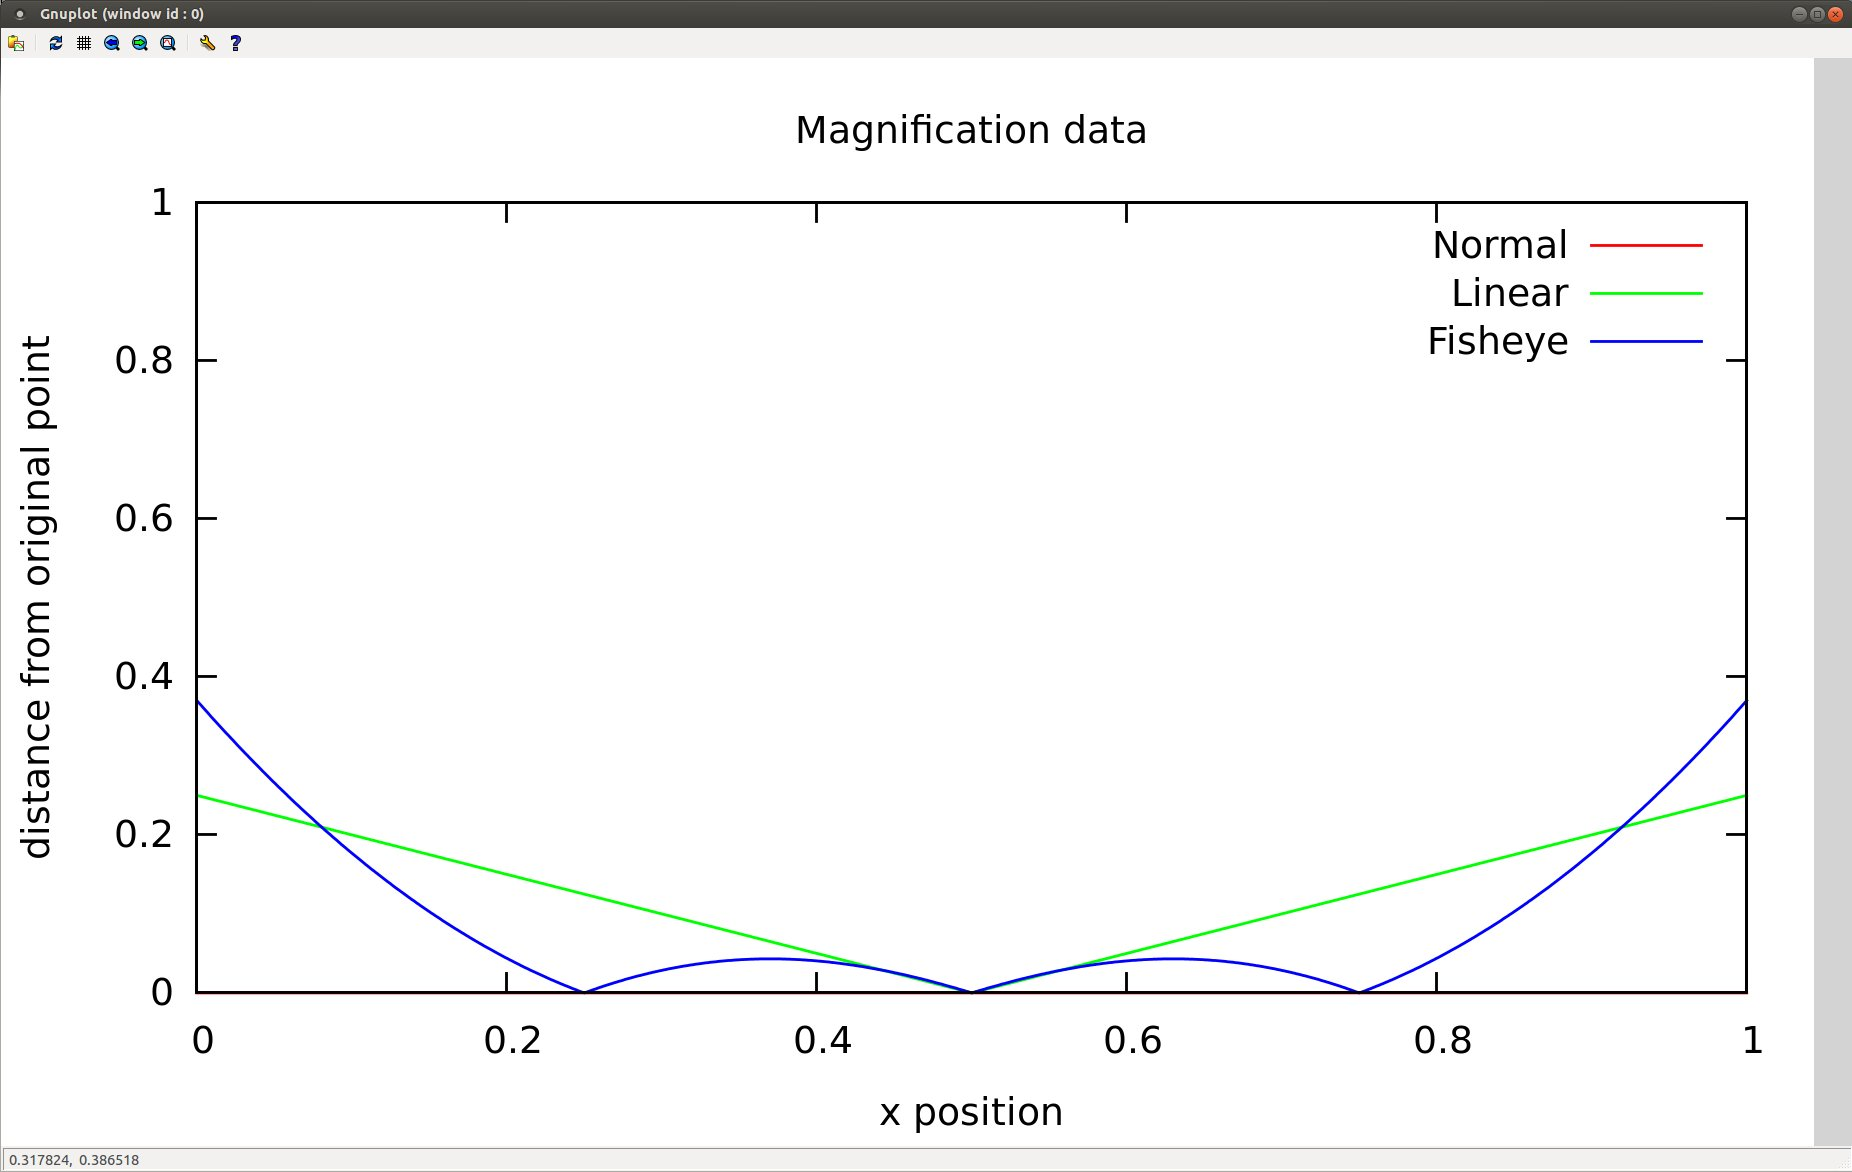
\includegraphics[width=2.8in]{figures/graph.jpg}
	\caption{The graph of distances from the transformed point to the original
    point, y is kept constant at 0.5}
	\label{fig:graph}
\end{figure}

Figure~\ref{fig:graph} shows a mathematical explanation of the constants for the linear
transformation radius, the fisheye transformation radius, the power of the
both transformations. Intersections between lines indicate that the
transformations produce the same point, and as such, present a relatively
distortion free zone for switching from one type of transformation to another.

The fact that this central feature must be computed before even
running the program is a major flaw in the current system.

\begin{figure}
	\centering
	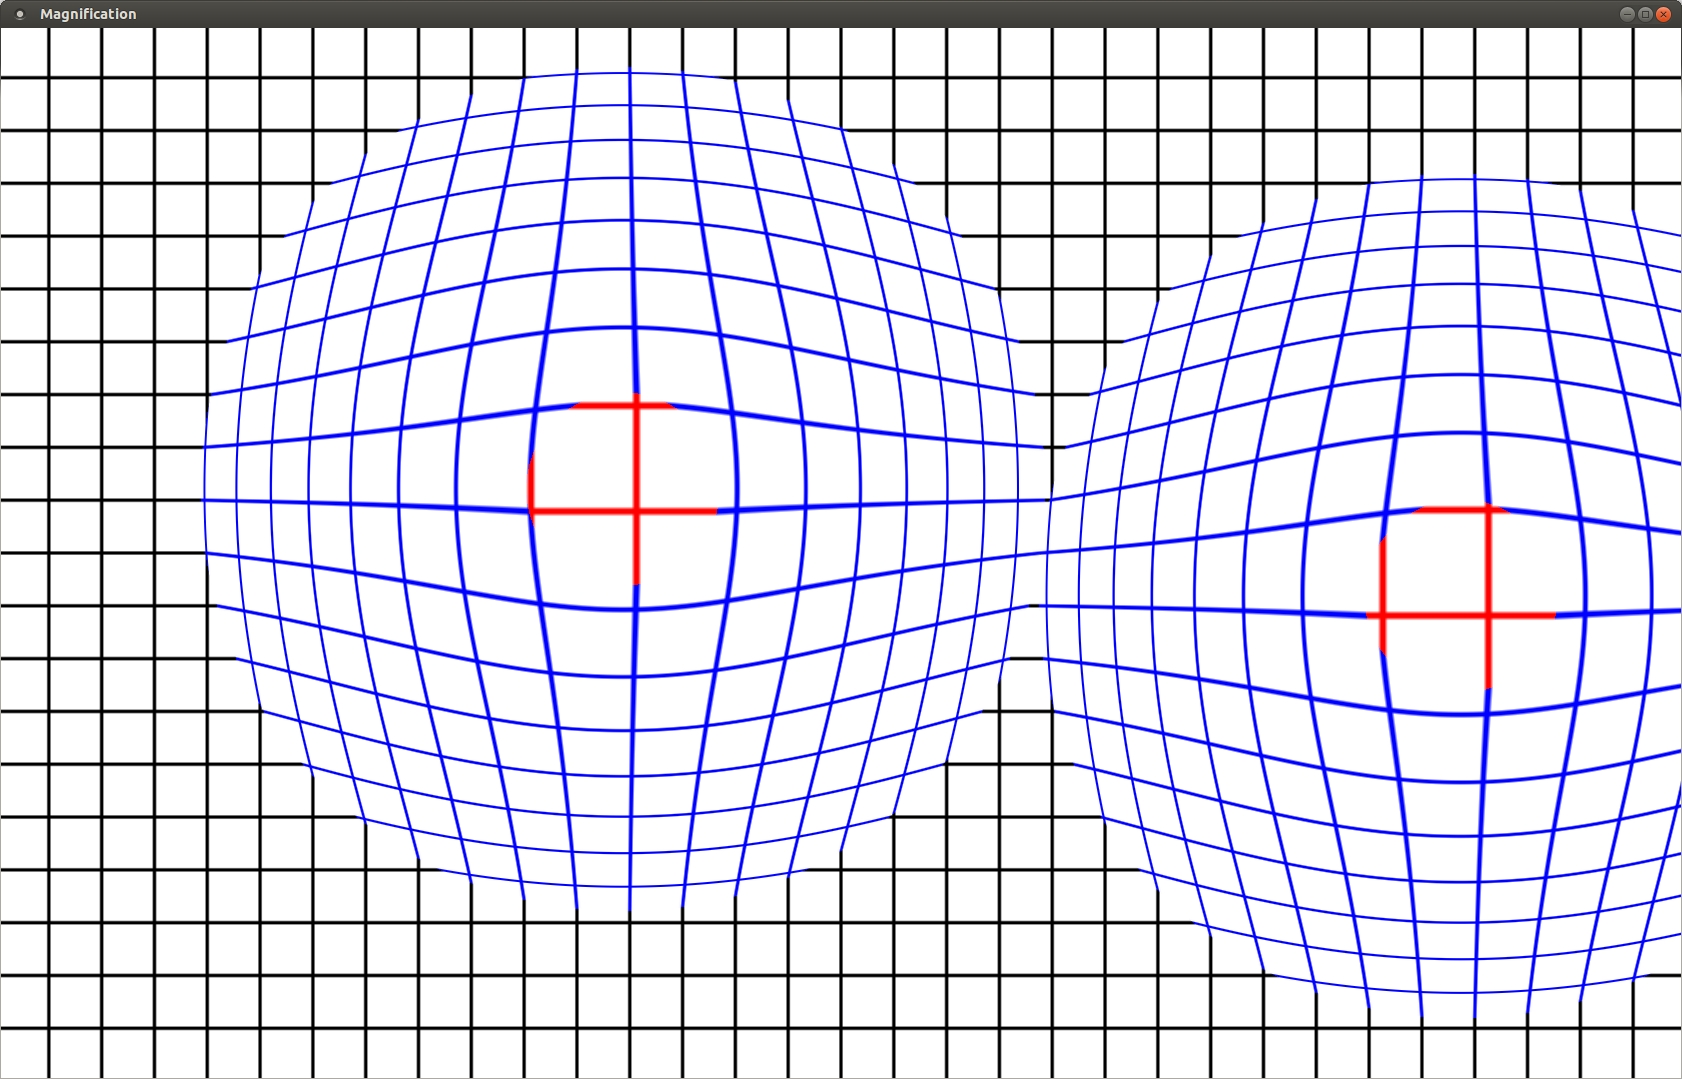
\includegraphics[width=2.8in]{figures/tangent.jpg}
	\caption{Two magnification areas tangent to one another.}
	\label{fig:tangent}
\end{figure}
\begin{figure}
	\centering
	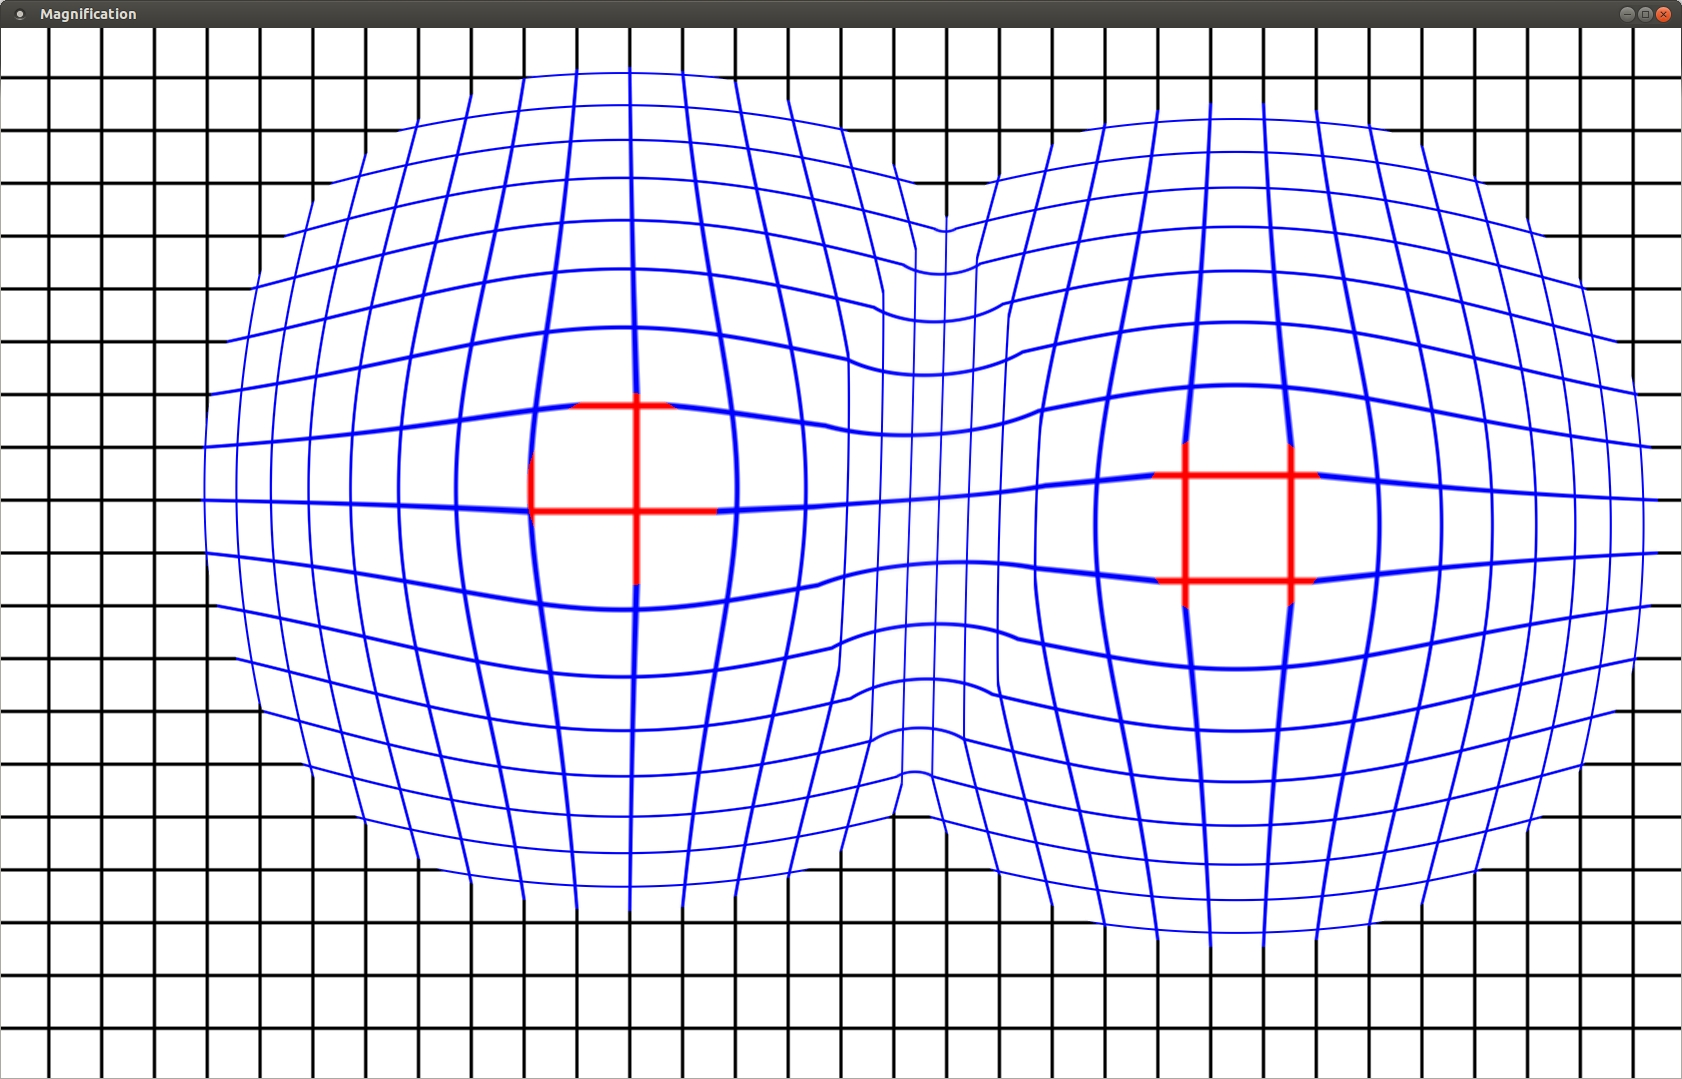
\includegraphics[width=2.8in]{figures/outer.jpg}
	\caption{Two magnification areas with just the fisheye
    transformations interacting}
	\label{fig:outer}
\end{figure}
\begin{figure}
	\centering
	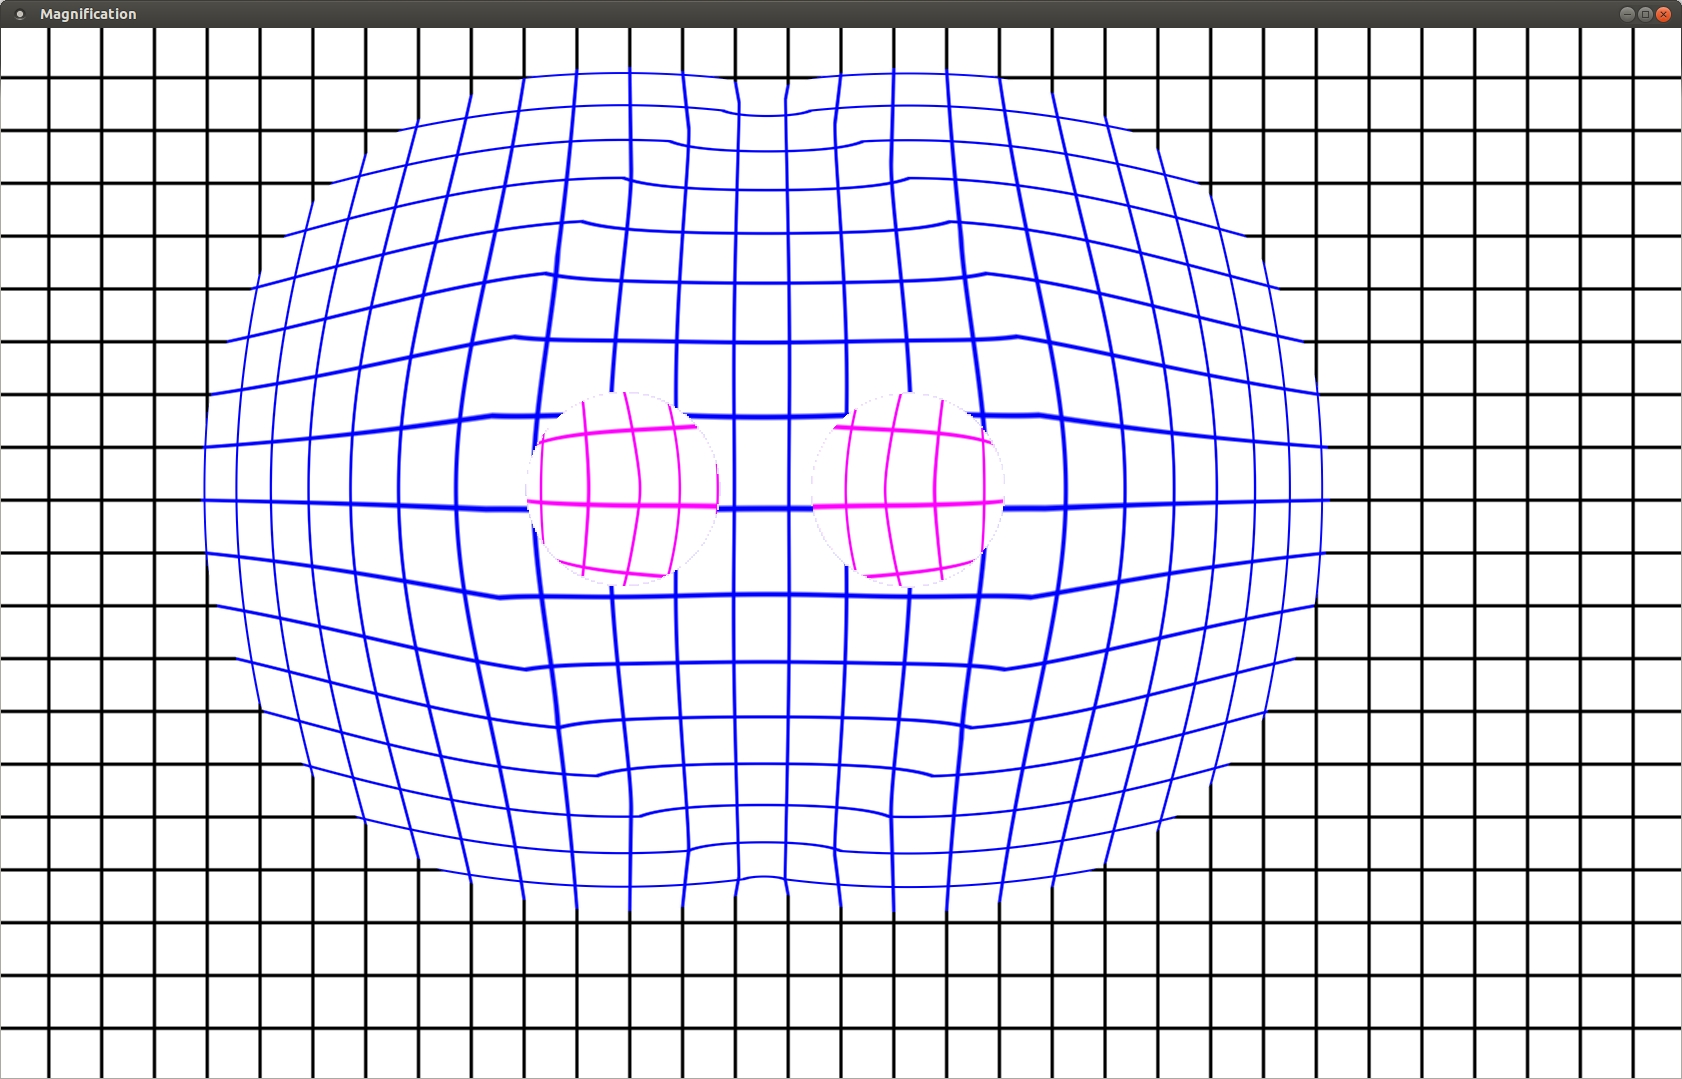
\includegraphics[width=2.8in]{figures/inner_and_outer.jpg}
	\caption{Two magnification areas with the fisheye and
    linear transformations interacting.}
	\label{fig:inner_and_outer}
\end{figure}
\begin{figure}
	\centering
	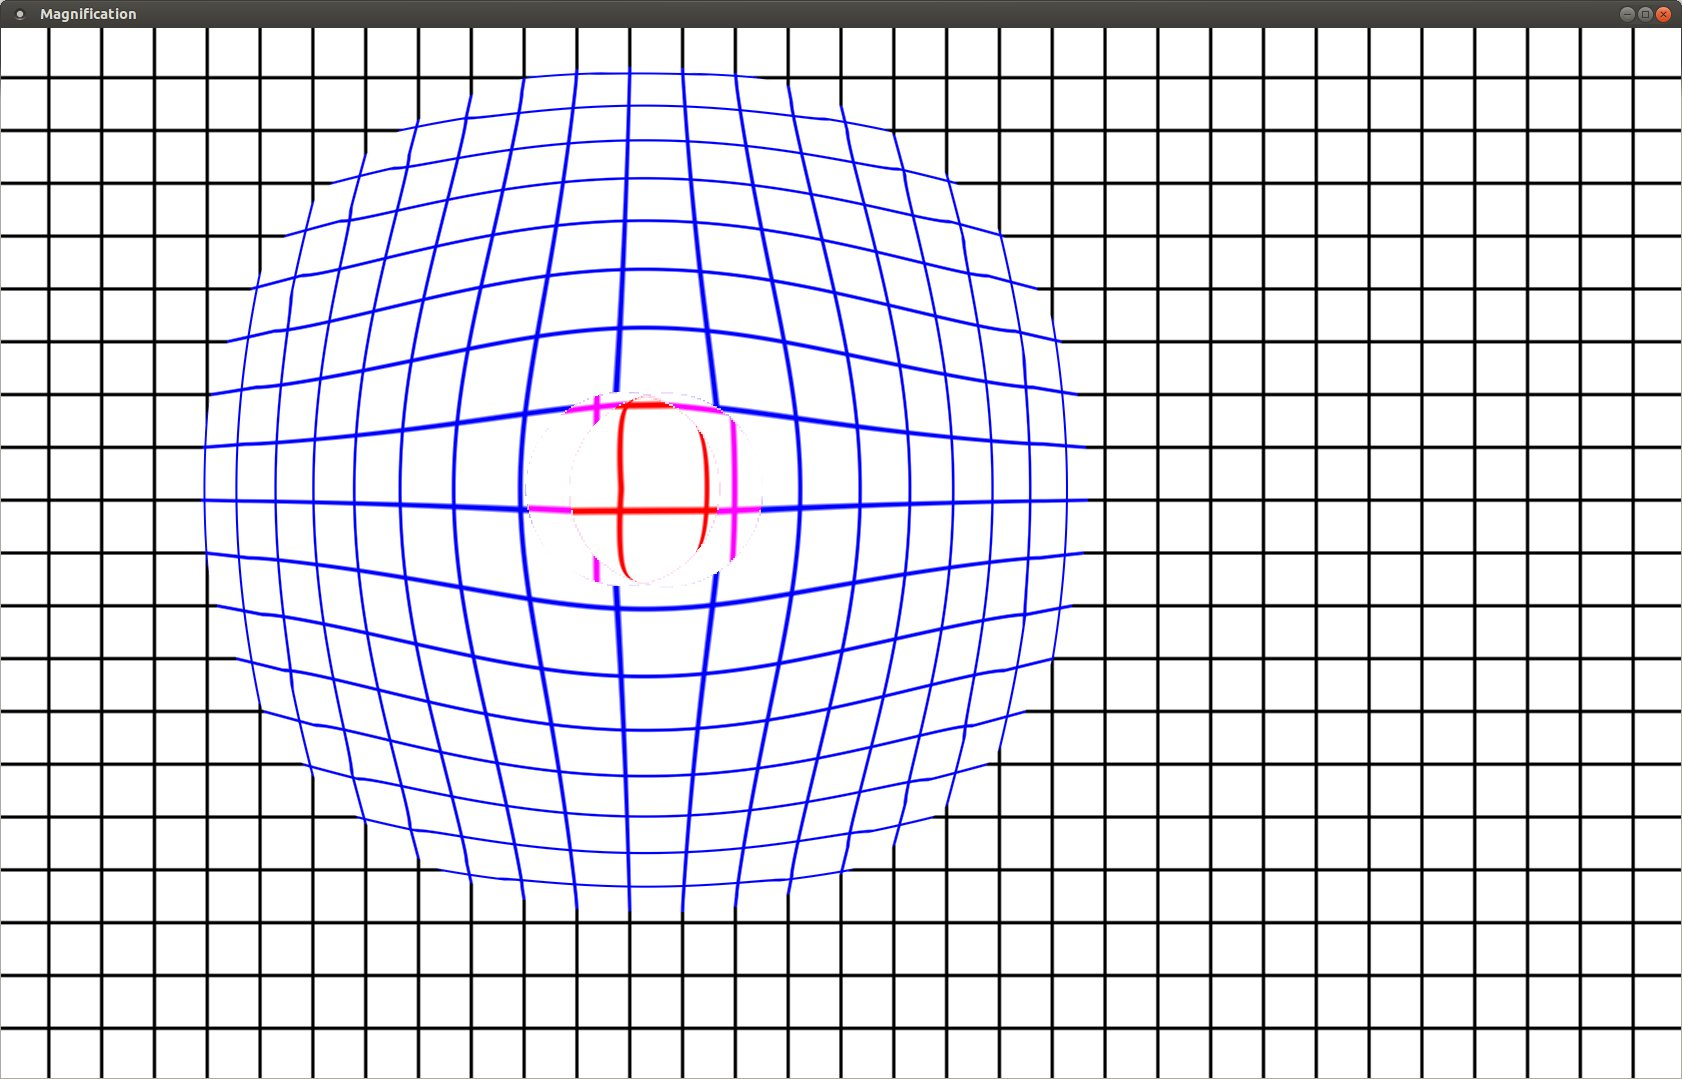
\includegraphics[width=2.8in]{figures/inner_and_inner.jpg}
	\caption{Two magnification areas with the linear transformations
    interacting.}
	\label{fig:inner_and_inner}
\end{figure}
\begin{figure}
	\centering
	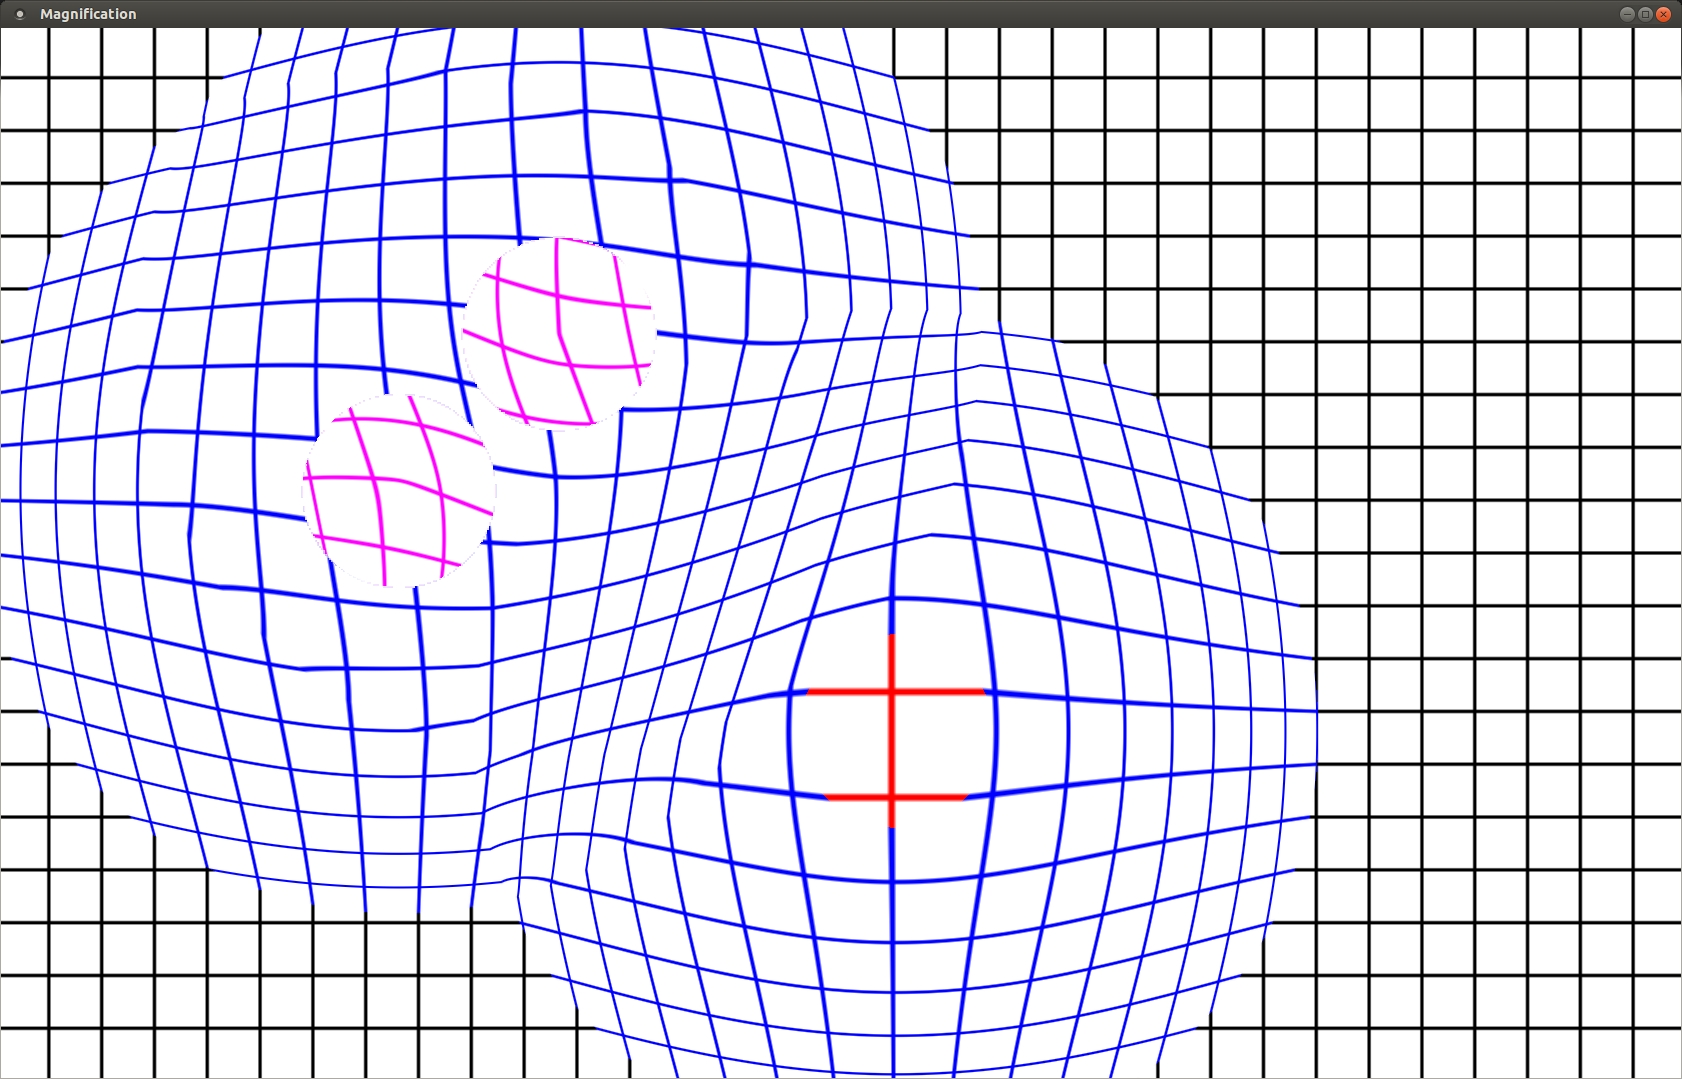
\includegraphics[width=2.8in]{figures/multiple.jpg}
	\caption{Three magnification areas interacting.}
	\label{fig:multiple}
\end{figure}

Figures~\ref{fig:tangent} through~\ref{fig:multiple} all show different interactions 
between the multiple magnification regions. Blue regions indicate that the lines
have been transformed by only the fisheye transformation, red regions indicate
that the liens have been transformed by only the linear transformation, and
purple areas indicate that it has been transformed by a mixture of both.

Figures~\ref{fig:tangent} and~\ref{fig:outer} show that if the only interactions 
between the magnification regions occur with the fisheye transformations, the 
resulting image contains $C^0$ continuity.

Other figures show that the simple linear weighted average algorithm of combining
magnification areas causes the resulting figure to be $C^{-1}$ continuous. 
Figure~\ref{fig:inner_and_outer} shows that simple interactions between the linear
and magnification area only result in slight disturbances for the formerly 
linear areas. Figure~\ref{fig:inner_and_inner} also displays some errors
with the linear transformation region, as the red highlighted area should
be completely straight lines.

Figure~\ref{fig:multiple} shows that the model for fisheye transformations
remains $C^0$ continuous even among multiple magnification regions.

Various different forms of the nonlinear transformations were attempted
with limited success. The initial proposal by Sarkar et al.\ is orthogonal
in nature; attempts to convert the equation to a polar coordinate system
to allow for a radial magnification did not produce good results. 

\subsection{Performance}
Currently, with a window size of 1680 x 1050, a 3.1 MB source texture of 
1024 x 1024, the program runs in real time with up to 15 computer-controlled
cursors and one human controlled cursor.

The current implementation of the cursor system may need to be reworked
in the future due to its current inefficiency in OpenGL contexts. Constant
frame by frame updates of a subsection of a VBO may result in inefficiencies,
a better implementation would use instanced rendering. This may be a non-issue
due to the simple fact that few more than a dozen users would likely be
interacting with the system at any given point in time. 

\section{Conclusion}
In conclusion, the linear averaging of different types of transformations
presents the possibility for a new method of viewing multiple areas
of interest within a graphical visualization.

Similarly, this paper has also shown the limitations of using simple
combinations of various transformation functions to present this type of
data. Being unable to easily change the linear magnification levels or the
radii of the two transformation areas severely detriment the usefulness
of the overall application.

It has been shown that even with a decent number of users participating
in this system, the application can still perform in real-time with
simulated users. This may change when multiple users interact with a
system depending on the overall implementation.

\section{Future Work}
While the current application has a limited amount of functionality, it
has also laid the groundwork for many possible modifications.

\subsection{Adaptive Parameters}
One of the largest flaws with the current system is its required and
partially incorrect values for the linear and nonlinear magnification
regions.

A large portion of time needs to be invested in evaluating more methods
of generating a blended function from the area of no local magnification
to areas of possibly extreme linear magnification. The limitations of such
a system have been hinted at by Keahey et al. They claimed that the area
of linear zoom is directly proportional to the radius of the inner zoom.
\cite{kr96}

\subsection{Global Zooming}
As explained before, the current system does not have global zooming, though
a previous iteration of the simulation had a working implementation without
multiple cursors. Any future work with regards to this area will be forced
to cause the cursors to move when the magnification changes to prevent 
continual zooming in or zooming out with relation to a specific focal point.

\subsection{Merging of Regions}
The behavior of these merged regions is currently only affected by the
linear weighted average of the new UV coordinates. There may be cases
where the more useful visualization would be to combine nearby
areas of magnification into larger regions. 

This overall magnification scheme has many problems, as the threshold
for combining magnifications is currently abrupt. There may also be
situations where combining nearby regions causes a chain reaction
as the larger regions combine recursively. Whether this behavior
is acceptable or not will depend highly upon user feedback.

In cases where two regions are extremely close to one another, another
solution may be to simply disregard the self enforced restriction
of desiring distortion-free areas. 

\subsection{Integration with Existing Systems}
The current application only deals with a simple 2D texture being mapped
onto a single pair of triangles that form a square. Much work will
go into integrating this with existing systems for usage in map
visualization. This will require many changes to the overall system,
as the main map visualization requires many levels of zoom to produce
relevant information. Translating UV coordinates across boundaries
will also likely cause a problem with sampling the correct data.

The map visualization program also has many layers of data that
are important to a user. Performance problems may occur from changing
the existing system. One solution to the integration would be to 
have all data write to an intermediate frame buffer object (FBO) within
OpenGL and then perform the required transformations on the intermediate
data. This would also require the transformations to occur on the CPU
in order to move the interactive elements. Whether these new developments
would cause major performance or interaction problems remains to be seen.

The overall simulation currently only has one source of user input,
integrating this with both multiple mouse cursors and laser pointers
may require tuning with regards to global zoom functionality.

\bibliographystyle{acmsiggraph} 
\bibliography{writeup}

\end{document}
